% Options for packages loaded elsewhere
\PassOptionsToPackage{unicode}{hyperref}
\PassOptionsToPackage{hyphens}{url}
\PassOptionsToPackage{dvipsnames,svgnames*,x11names*}{xcolor}
%
\documentclass[
  12pt,
]{article}
\usepackage{amsmath,amssymb}
\usepackage{lmodern}
\usepackage{setspace}
\usepackage{iftex}
\ifPDFTeX
  \usepackage[T1]{fontenc}
  \usepackage[utf8]{inputenc}
  \usepackage{textcomp} % provide euro and other symbols
\else % if luatex or xetex
  \usepackage{unicode-math}
  \defaultfontfeatures{Scale=MatchLowercase}
  \defaultfontfeatures[\rmfamily]{Ligatures=TeX,Scale=1}
  \setmainfont[]{Georgia}
\fi
% Use upquote if available, for straight quotes in verbatim environments
\IfFileExists{upquote.sty}{\usepackage{upquote}}{}
\IfFileExists{microtype.sty}{% use microtype if available
  \usepackage[]{microtype}
  \UseMicrotypeSet[protrusion]{basicmath} % disable protrusion for tt fonts
}{}
\makeatletter
\@ifundefined{KOMAClassName}{% if non-KOMA class
  \IfFileExists{parskip.sty}{%
    \usepackage{parskip}
  }{% else
    \setlength{\parindent}{0pt}
    \setlength{\parskip}{6pt plus 2pt minus 1pt}}
}{% if KOMA class
  \KOMAoptions{parskip=half}}
\makeatother
\usepackage{xcolor}
\IfFileExists{xurl.sty}{\usepackage{xurl}}{} % add URL line breaks if available
\IfFileExists{bookmark.sty}{\usepackage{bookmark}}{\usepackage{hyperref}}
\hypersetup{
  colorlinks=true,
  linkcolor={Maroon},
  filecolor={Maroon},
  citecolor={Blue},
  urlcolor={blue},
  pdfcreator={LaTeX via pandoc}}
\urlstyle{same} % disable monospaced font for URLs
\usepackage[margin=1.0in]{geometry}
\usepackage{graphicx}
\makeatletter
\def\maxwidth{\ifdim\Gin@nat@width>\linewidth\linewidth\else\Gin@nat@width\fi}
\def\maxheight{\ifdim\Gin@nat@height>\textheight\textheight\else\Gin@nat@height\fi}
\makeatother
% Scale images if necessary, so that they will not overflow the page
% margins by default, and it is still possible to overwrite the defaults
% using explicit options in \includegraphics[width, height, ...]{}
\setkeys{Gin}{width=\maxwidth,height=\maxheight,keepaspectratio}
% Set default figure placement to htbp
\makeatletter
\def\fps@figure{htbp}
\makeatother
\setlength{\emergencystretch}{3em} % prevent overfull lines
\providecommand{\tightlist}{%
  \setlength{\itemsep}{0pt}\setlength{\parskip}{0pt}}
\setcounter{secnumdepth}{-\maxdimen} % remove section numbering
\usepackage{longtable}
\usepackage{graphicx}
\usepackage{booktabs}
\usepackage{textcomp}
\usepackage{xcolor}
\usepackage{colortbl}
\usepackage{geometry}
\usepackage{subcaption}
\usepackage{lineno}
\usepackage{makecell}
\usepackage{pdflscape}
\definecolor{listcomment}{rgb}{0.0,0.5,0.0}
\definecolor{listkeyword}{rgb}{0.0,0.0,0.5}
\definecolor{listnumbers}{gray}{0.65}
\definecolor{listlightgray}{gray}{0.955}
\definecolor{listwhite}{gray}{1.0}
\ifLuaTeX
  \usepackage{selnolig}  % disable illegal ligatures
\fi
\newlength{\cslhangindent}
\setlength{\cslhangindent}{1.5em}
\newlength{\csllabelwidth}
\setlength{\csllabelwidth}{3em}
\newenvironment{CSLReferences}[2] % #1 hanging-ident, #2 entry spacing
 {% don't indent paragraphs
  \setlength{\parindent}{0pt}
  % turn on hanging indent if param 1 is 1
  \ifodd #1 \everypar{\setlength{\hangindent}{\cslhangindent}}\ignorespaces\fi
  % set entry spacing
  \ifnum #2 > 0
  \setlength{\parskip}{#2\baselineskip}
  \fi
 }%
 {}
\usepackage{calc}
\newcommand{\CSLBlock}[1]{#1\hfill\break}
\newcommand{\CSLLeftMargin}[1]{\parbox[t]{\csllabelwidth}{#1}}
\newcommand{\CSLRightInline}[1]{\parbox[t]{\linewidth - \csllabelwidth}{#1}\break}
\newcommand{\CSLIndent}[1]{\hspace{\cslhangindent}#1}

\author{}
\date{\vspace{-2.5em}}

\begin{document}

\setstretch{1.5}
\linenumbers
\pagenumbering{gobble}

\setstretch{1}

\begin{centering}

$ $

\vspace{6cm}

\LARGE

{\bf The ANTsX Ecosystem for Spatiotemporal Mapping of the Mouse Brain}

\vspace{1.0 cm}

\normalsize

Nicholas J. Tustison$^{1}$,
Min Chen$^{2}$,
Fae N. Kronman$^{3}$,
Jeffrey T. Duda$^{2}$,
Clare Gamlin$^{4}$,
Lydia Ng$^{4}$,
Yongsoo Kim$^{3}$, and
James C. Gee$^{2}$

\small

$^{1}$Department of Radiology and Medical Imaging, University of Virginia, Charlottesville, VA \\
$^{2}$Department of Radiology, University of Pennsylvania, Philadelphia, PA \\
$^{3}$Department of Neural and Behavioral Sciences, Penn State University, Hershey, PA \\
$^{4}$Allen Institute for Brain Science, Seattle, WA \\

\vspace{1.5 cm}

\end{centering}

\vspace{5.5 cm}

\noindent

\rule{4cm}{0.4pt}

\scriptsize

Corresponding author:\\
Nicholas J. Tustison, DSc\\
Department of Radiology and Medical Imaging\\
University of Virginia\\
\href{mailto:ntustison@virginia.edu}{\nolinkurl{ntustison@virginia.edu}}

\normalsize

\newpage

\setstretch{1.5}

\hypertarget{abstract}{%
\section*{Abstract}\label{abstract}}
\addcontentsline{toc}{section}{Abstract}

Precision mapping techniques coupled with high resolution image
acquisition of the mouse brain permit the study of the spatial
organization of gene activity and their mutual interaction for a
comprehensive view of salient structural/functional relationships. Such
research is facilitated by standardized anatomical coordinate systems,
such as the well-known Allen Common Coordinate Framework version 3
(CCFv3), and the ability to map to such reference atlases. The Advanced
Normalization Tools Ecosystem (ANTsX) is a comprehensive open-source
software image analysis toolkit with applicability to multiple organ
systems, modalities, and animal species. Herein, we illustrate the
utility of ANTsX for generating precision spatial mappings of the mouse
brain of different developmental ages including the prerequisite
preprocessing steps. Additionally, as a further illustration of ANTsX
capabilities, we use these publicly available mouse brain atlases to
generate a velocity flow-based mapping encompassing the entire
developmental trajectory, which we also make available to the public.

\clearpage

\hypertarget{introduction}{%
\section*{Introduction}\label{introduction}}
\addcontentsline{toc}{section}{Introduction}

Over the past two decades there has been a notable increase in
significant advancements in mesoscopic analysis of the mouse brain. It
is now possible to track single cell neurons in 3-D across full mouse
brains,\textsuperscript{1} observe whole brain developmental changes on
a cellular level,\textsuperscript{2} associate brain regions and tissues
with their genetic composition,\textsuperscript{3} and locally
characterize neural connectivity.\textsuperscript{4} Much of this
scientific achievement has been made possible due to breakthroughs in
high resolution imaging techniques that permit submicron, 3-D imaging of
whole mouse brains. Associated research techniques such as micro-optical
sectioning tomography,\textsuperscript{6} tissue
clearing,\textsuperscript{1,7} spatial
transcriptomics\textsuperscript{9} are all well-utilized in the course
of scientific investigations of mesoscale relationships in the mouse
brain.

An important component of these research programs is the ability to map
the various image data to anatomical reference
frames\textsuperscript{11} for inferring spatial relationships between
structures, cells, and genetics in the brain. This has motivated the
development of detailed structural image atlases of the mouse brain.
Notable examples include the Allen Brain Atlas and Coordinate
Frameworks\textsuperscript{13} and the Waxholm
Space.\textsuperscript{14} Despite the significance of these
contributions, challenges still exist in large part due to the wide
heterogeneity in associated study-specific image data. Variance in the
acquisition methods can introduce artifacts such as tissue distortion,
holes, bubbles, folding, tears, and missing slices. These severely
complicate assumed correspondence for registration.

To address such challenges, several software packages have been
developed over the years comprising solutions of varying
comprehensibility, sophistication, and availability. An early
contribution to the community was the Rapid Automatic Tissue
Segmentation (RATS) package\textsuperscript{15} for brain extraction
(available upon request). Of the publicly available packages, most, if
not all rely on well-established package dependencies originally
developed on human brain data. Another early tool was
SPMMouse\textsuperscript{16} based on the well-known Statistical
Parametric Mapping (SPM) software package.\textsuperscript{17} The
automated mouse atlas propagation (aMAP) tool is largely a front-end for
the NiftyReg image registration package\textsuperscript{18} applied to
mouse data which is currently available as a Python
module.\textsuperscript{19} NiftyReg is also used by the Atlas-based
Imaging Data Analysis (AIDA) MRI pipeline\textsuperscript{20} as well as
the Multi Atlas Segmentation and Morphometric Analysis Toolkit (MASMAT).
Whereas the former also incorporates the FMRIB Software Library
(FSL)\textsuperscript{21} for brain extraction and
DSIStudio\textsuperscript{22} for DTI processing, the latter uses
NiftySeg and multi-consensus labeling tools\textsuperscript{23} for
brain extraction and parcellation. In addition, MASMAT incorporates N4
bias field correction\textsuperscript{24} from the Advanced
Normalization Tools Ecosystem (ANTsX)\textsuperscript{25} as do the
packages Multi-modal Image Registration And Connectivity anaLysis
(MIRACL),\textsuperscript{26} Sammba-MRI,\textsuperscript{27} and Small
Animal Magnetic Resonance Imaging (SAMRI).\textsuperscript{28} However,
whereas Saamba-MRI uses AFNI\textsuperscript{29} for image registration;
MIRACL, SAMRI, and BrainsMapi\textsuperscript{30} all use ANTsX tools
for computing image-based correspondences. Other packages use
landmark-based approaches to image registration including
SMART---\textsuperscript{31}an R package for semi-automated
landmark-based registration and segmentation of mouse brain based on
WholeBrain.\textsuperscript{32} FriendlyClearMap\textsuperscript{33}
uses the landmark-based registration functionality of
Elastix.\textsuperscript{34} Finally, the widespread adoption of deep
learning techniques has also influenced development in mouse brain
imaging methodologies. For example, if tissue deformations are not
considered problematic for a particular dataset, DeepSlice can be used
to determine affine mappings\textsuperscript{35} with the optimal
computational efficiency associated with neural networks.

\hypertarget{the-antsx-ecosystem}{%
\subsubsection*{The ANTsX Ecosystem}\label{the-antsx-ecosystem}}
\addcontentsline{toc}{subsubsection}{The ANTsX Ecosystem}

As noted above, many of the existing approaches for processing of mouse
brain image data use ANTsX tools for core steps in various workflows,
particularly its pairwise, intensity-based image registration tools and
bias field correction. Historically, ANTsX development is originally
based on fundamental approaches to image
mapping,\textsuperscript{36--38} particularly in the human brain, which
has resulted in core contributions to the field such as the well-known
and highly-vetted Symmetric Normalization (SyN)
algorithm.\textsuperscript{39} Since its development, various
independent platforms have been used to evaluate ANTsX image
registration capabilities in the context of different application foci
which include multi-site brain MRI data,\textsuperscript{40} pulmonary
CT data,\textsuperscript{41} and most recently multi-modal brain
registration in the presence of tumors.\textsuperscript{42}


\begin{table}
  \small
   \centering
   \vspace{-0.25cm}
   \caption{Sampling of ANTsX functionality} 
   \begin{tabular*}{0.95\textwidth}{l @{\extracolsep{\fill}} p{.575\textwidth}}
    \toprule
    \multicolumn{2}{c}{\cellcolor{gray!25} \em ANTsPy: Preprocessing} \\
    \cmidrule[1pt](lr){1-2}
    bias field correction & \texttt{n4\_bias\_field\_correction(...)} \\
    image denoising  & \texttt{denoise\_image(...)} \\
    \cmidrule[1pt](lr){1-2}
    \multicolumn{2}{c}{\cellcolor{gray!25} \em ANTsPy: Registration} \\
    \cmidrule[1pt](lr){1-2}
    image registration & \texttt{registration(...)} \\
    template generation  & \texttt{build\_template(...)} \\
    landmark registration & \texttt{fit\_transform\_to\_paired\_points(...)} \\
    time-varying landmark reg. & \texttt{fit\_time\_varying\_transform\_to\_point\_sets(...)} \\
    integrate velocity field & \texttt{integrate\_velocity\_field(...)} \\
    invert displacement field & \texttt{invert\_displacement\_field(...)} \\
    \cmidrule[1pt](lr){1-2}
    \multicolumn{2}{c}{\cellcolor{gray!25} \em ANTsPy: Segmentation} \\
    \cmidrule[1pt](lr){1-2}
    General segmentation & \texttt{atropos(...)} \\
    Joint label fusion & \texttt{joint\_label\_fusion(...)} \\
    diffeormorphic thickness   & \texttt{kelly\_kapowski(...)} \\
    \cmidrule[1pt](lr){1-2}
    \multicolumn{2}{c}{\cellcolor{gray!25} \em ANTsPy: Miscellaneous} \\
    \cmidrule[1pt](lr){1-2}
    Regional intensity statistics & \texttt{label\_stats(...)} \\
    Regional shape measures & \texttt{label\_geometry\_measures(...)} \\
    B-spline approximation & \texttt{fit\_bspline\_object\_to\_scattered\_data(...)} \\
    Visualize images and overlays\,\,\,\,\,\,\,\,\,\,\,\, & \texttt{plot(...)} \\
    \cmidrule[1pt](lr){1-2}
    \multicolumn{2}{c}{\cellcolor{gray!25} \em ANTsPyNet} \\
    \cmidrule[1pt](lr){1-2}
    brain extraction & \texttt{mouse\_brain\_extraction(...modality="t2"...)} \par \texttt{mouse\_brain\_extraction(...modality="ex5"...)} \\
    foreground extraction & \texttt{mouse\_histology\_brain\_mask(...)} \\
    midline segmentation & \texttt{mouse\_histology\_hemispherical\_coronal\_mask(...)} \\
    cerebellum segmentation & \texttt{mouse\_histology\_cerebellum\_mask(...)} \\
    super resolution & \texttt{mouse\_histology\_super\_resolution(...)} \\
    \bottomrule
    \multicolumn{2}{l}{\makecell[l]{
     \vspace{-3pt}
     \scriptsize ANTsX provides state-of-the-art open-science functionality for processing image data.  Such tools, including deep \\
     \vspace{-3pt}
     \scriptsize learning networks, support a variety of mapping-related tasks.  A more comprehensive listing of ANTsX tools with \\
     \vspace{-3pt}
     \scriptsize self-contained R and Python examples is provided as a gist page on GitHub (\url{https://tinyurl.com/antsxtutorial}). }
    }
   \end{tabular*}
 \label{table:methods}
\end{table}


Apart from its registration capabilities, ANTsX is a comprehensive
biological and medical image analysis toolkit, that comprises additional
functionality such as template generation, general data approximation,
and deep learning networks specifically trained for mouse data (see
Table \ref{table:methods}). The collective use of the toolkit has
demonstrated superb performance in multiple application areas (e.g.,
consensus labeling,\textsuperscript{43} brain tumor
segmentation,\textsuperscript{44} and cardiac motion
estimation).\textsuperscript{45} Importantly, ANTs is built on the
Insight Toolkit (ITK)\textsuperscript{46} deriving benefit from a very
capable open-source community of scientists and programmers as well as
providing a visible, open-source venue for algorithmic contributions.

\begin{figure}[!htb]
\centering
\makebox[\textwidth][c]{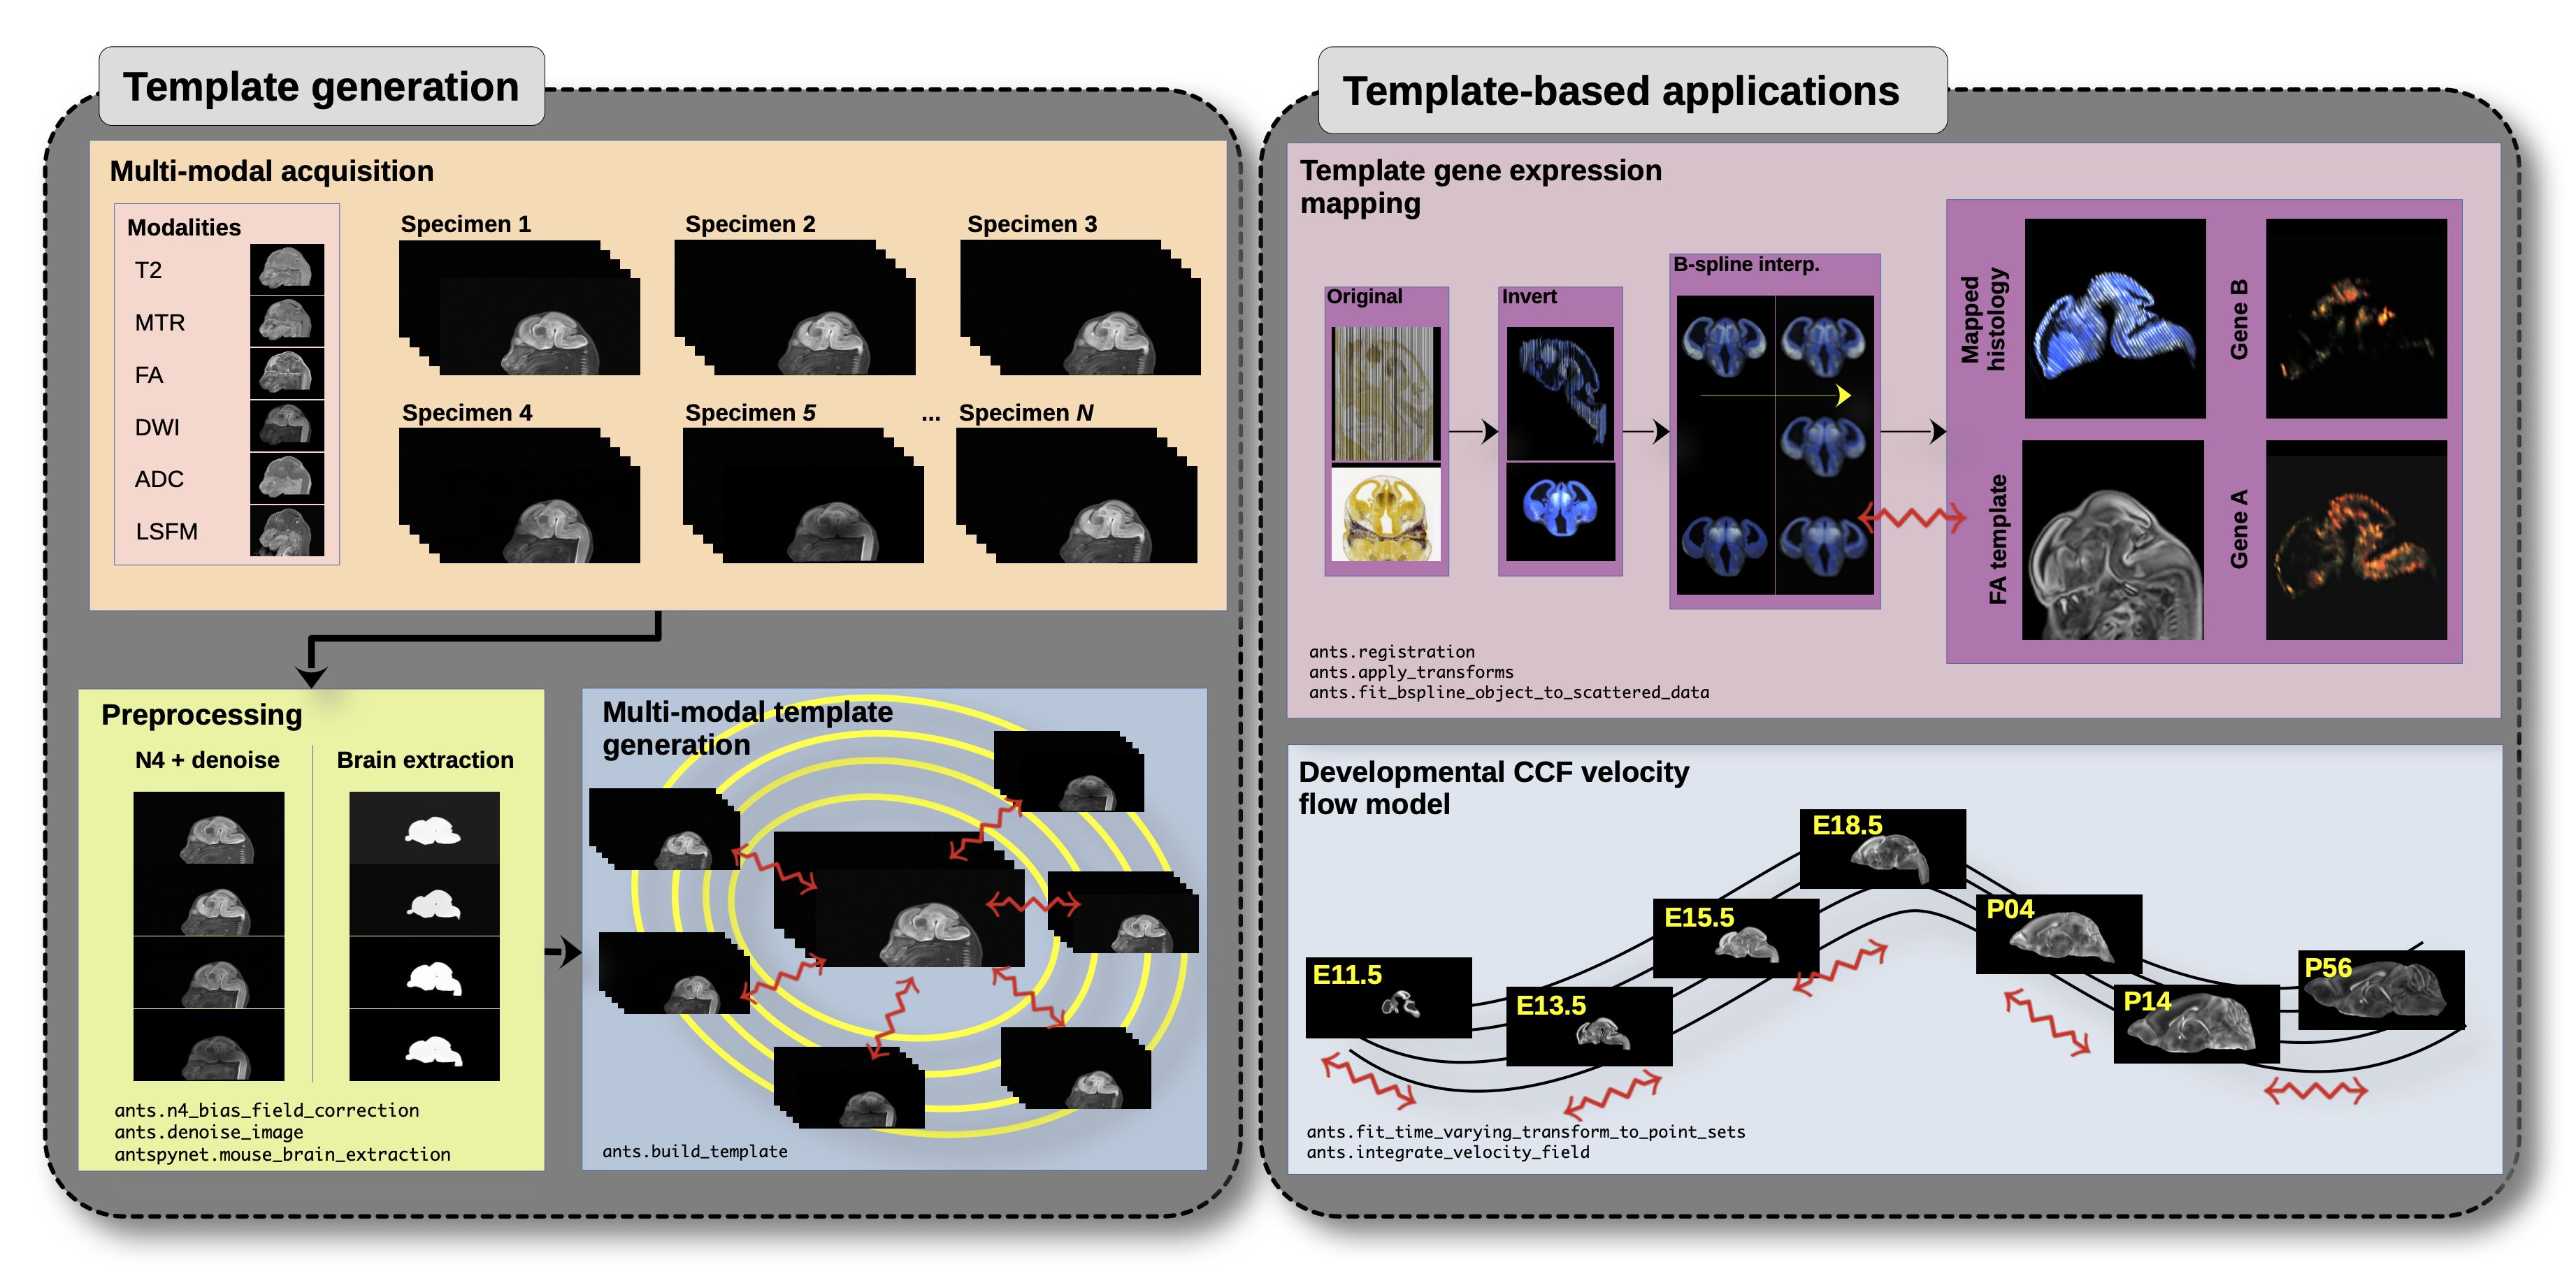
\includegraphics[width=1.2\textwidth]{Figures/pipeline3.png}}%
\caption{Illustration of a mouse brain template generation workflow and 
related template-based applications demonstrating the utility of different 
ANTsX tools.  After imaging acquisition of the study population, various 
preprocessing steps are applied to the imaging data such as bias correction,
denoising, and brain extraction as dictated by the needs of the study 
protocol.  Not shown is the possibility of template symmetrization by 
contralaterally flipping the image data associated with each specimen.  
In the case of the DevCCF, applications include gene expression mapping 
and the associated velocity flow model for pseudo-template generation.}
\label{fig:pipeline}
\end{figure}

Recently, the developmental common coordinate framework (DevCCF) was
introduced to the mouse brain research community as a public
resource.\textsuperscript{47} These symmetric atlases, comprising both
multimodal image data and anatomical segmentations defined by
developmental ontology, span the mouse embryonic days (E) 11.5, E13.5,
E15.5, E18.5 and postnatal day (P) 4, P14, and P56. Modalities include
at least four MRI contrasts and light sheet flourescence miscroscopy
(LSFM) per developmental stage. Gene expression and other cell type data
were mapped to the corresponding developmental time point to guide the
associated anatomical parcellations. To further demonstrate the
practical utility of the DevCCF, the P56 template was integrated with
the Allen CCFv3 for mapping spatial transcriptome cell-type data. These
processes, specifically template generation and multi-modal image
mapping, were performed using ANTsX functionality in the presence of
previously noted image mapping difficulties (e.g., missing slices,
tissue distortion) illustrated in Figure \ref{fig:pipeline}.

Given the temporal gaps in the discrete set of developmental atlases, we
augment the template generation explanation previously
given\textsuperscript{47} from a developer's perspective. We hope that
this will provide additional information for the interested reader for
potential future template generation. Related, we also provide a
complementary strategy for inferring correspondence and mapping
information within the temporally continuous domain spanned and sampled
by the existing set of embryonic and postnatal atlas brains of the
DevCCF. Recently developed ANTsX functionality include the generation of
a diffeomorphic velocity flow transformation model\textsuperscript{48}
spanning developmental stages where mappings between any two continuous
time points within the span bounded by the E11.5 and P56 atlases is
determined by integration of the generated time-varying velocity
field.\textsuperscript{49} Such transformations permit the possibility
of ``pseudo'' templates generated between available developmental
stages.

\clearpage
\newpage

\hypertarget{results}{%
\section*{Results}\label{results}}
\addcontentsline{toc}{section}{Results}

\hypertarget{template-building}{%
\subsection*{Template building}\label{template-building}}
\addcontentsline{toc}{subsection}{Template building}

Template building using ANTsX tools was first described
in.\textsuperscript{50} Subsequently, multi-modal and symmetrical
variants were more explicitly described as part of the brain tumor
segmentation approach.\textsuperscript{51}

\hypertarget{the-devccf-velocity-flow-model}{%
\subsection*{The DevCCF Velocity Flow
Model}\label{the-devccf-velocity-flow-model}}
\addcontentsline{toc}{subsection}{The DevCCF Velocity Flow Model}

To continuously link the DevCCF atlases, a velocity flow model was
constructed using Dev-CCF derived data and ANTsX functionality available
in both ANTsR and ANTsPy. Although many implementations optimize
variations of this transformtion model (and others) using various image
intensity similarity metrics, we opted to to implement a separate
determination of iterative correspondence and transformation
optimization. This decision was based on existing ANTsX functionality
and wanting complementary utility for the toolkit.

ANTsX, being built on top of ITK, uses an ITK image data structure for
the 4-D velocity field where each voxel contains the \(x\), \(y\), \(z\)
components of the field at that point. Field regularization is provided
by a novel B-spline scattered data approximation
technique\textsuperscript{52} which permits individual point-based
weighting. Both field regularization and integration of the velocity
field are built on ITK functions written by ANTsX developers.

The optimized velocity field described here is of size
\([256, 182, 360]\) (or \(50 \mu\)m isotropic) \(\times 11\) integration
points for a total compressed size of a little over 2 GB. This choice
represented weighing the trade-off between tractability, portability,
and accuracy. However, all data and code to reproduce the results
described are available in a dedicated GitHub repository
(\url{https://github.com/ntustison/DevCCF-Velocity-Flow}).

\hypertarget{data-preparation}{%
\subsubsection*{Data preparation}\label{data-preparation}}
\addcontentsline{toc}{subsubsection}{Data preparation}

\begin{figure}[!htb]
\centering
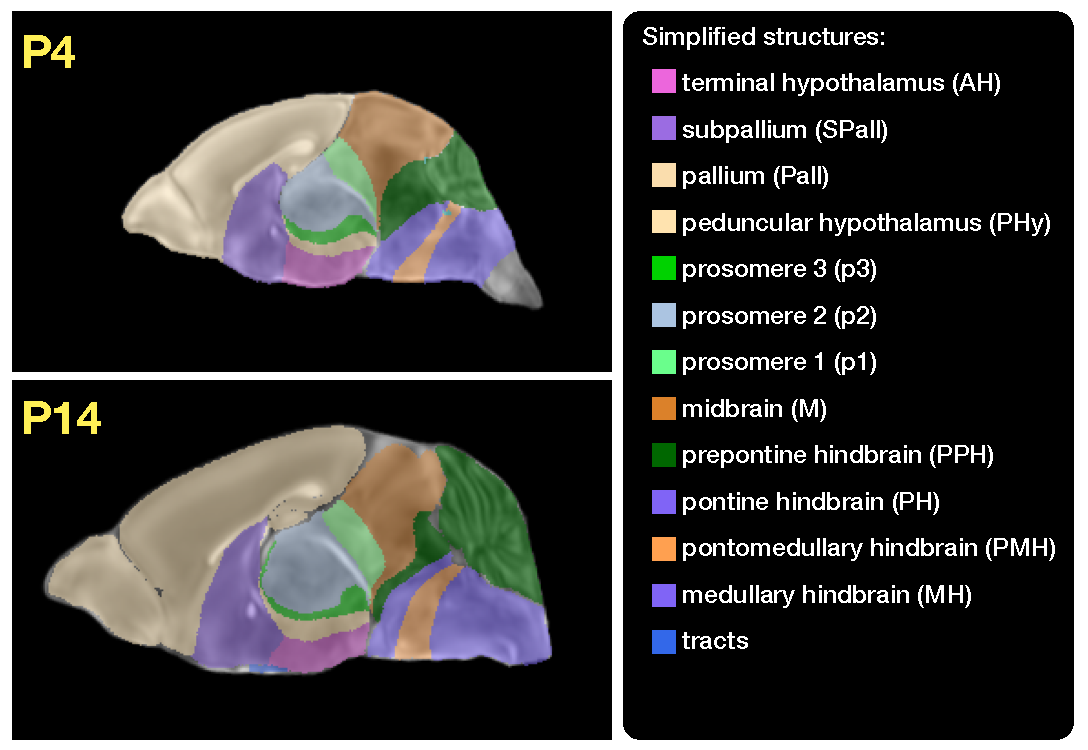
\includegraphics[width=0.75\textwidth]{Figures/SimplifiedAnnotations.pdf}
\caption{Annotated regions representing common labels across developmental stages which
are illustrated for both P4 and P14.}
\label{fig:simplifiedannotations}
\end{figure}

Labeled annotations are available as part of the original DevCCF and
reside in the space of each developmental template which range in
resolution from \(31.5-50 \mu\)m. Across all atlases, the total number
of labels exceeded 2500 without taken into account per hemispherical
enumeration. From this set of labels, there were a common set of 24
labels (12 per hemisphere) across all atlases that were used for
optimization and evaluation. These regions are illustrated for the P4
and P14 stages in Figure \ref{fig:simplifiedannotations}.

Prior to velocity field optimization, the data was rigidly transformed
to a common space. Using the centroids for the common label set of each
CCFDev atlas, the ANTsPy
\texttt{ants.fit\_transform\_to\_paired\_points(...)} function was used
to warp each atlas to the space of the P56 atlas and then downsampled to
\(50 \mu\)m isotropic resolution. In order to determine the common point
sets across stages, the multi-metric capabilities of
\texttt{ants.registration(...)} were used. Instead of performing
intensity-based pairwise registration directly on these multi-label
images, each label was used to construct a separate fixed and moving
image pair resulting in a multi-metric registration optimization
scenario involving 24 binary image pairs (each label weighted equally)
for optimizing correspondence between neighboring atlases using the mean
squares metric and the SyN transform.

To provide the common point sets across all seven developmental atlases,
the label boundaries and whole regions were sampled in the P56 atlas and
then propagated to each atlas using the transformations derived from the
pairwise registrations. Based on previous experience as both the
developers of users of these tools, we selected a sampling rate of 10\%
for the contour points and 1\% for the regional points for a total
number of points being per atlas being \(173303\)
(\(N_{contour} = 98151\) and \(N_{region}=75152\)). Boundary points were
weighted twice as those of regional points for the B-spline data
approximation optimization.

\hypertarget{optimization}{%
\subsubsection*{Optimization}\label{optimization}}
\addcontentsline{toc}{subsubsection}{Optimization}

\begin{figure}[!htb]
\centering
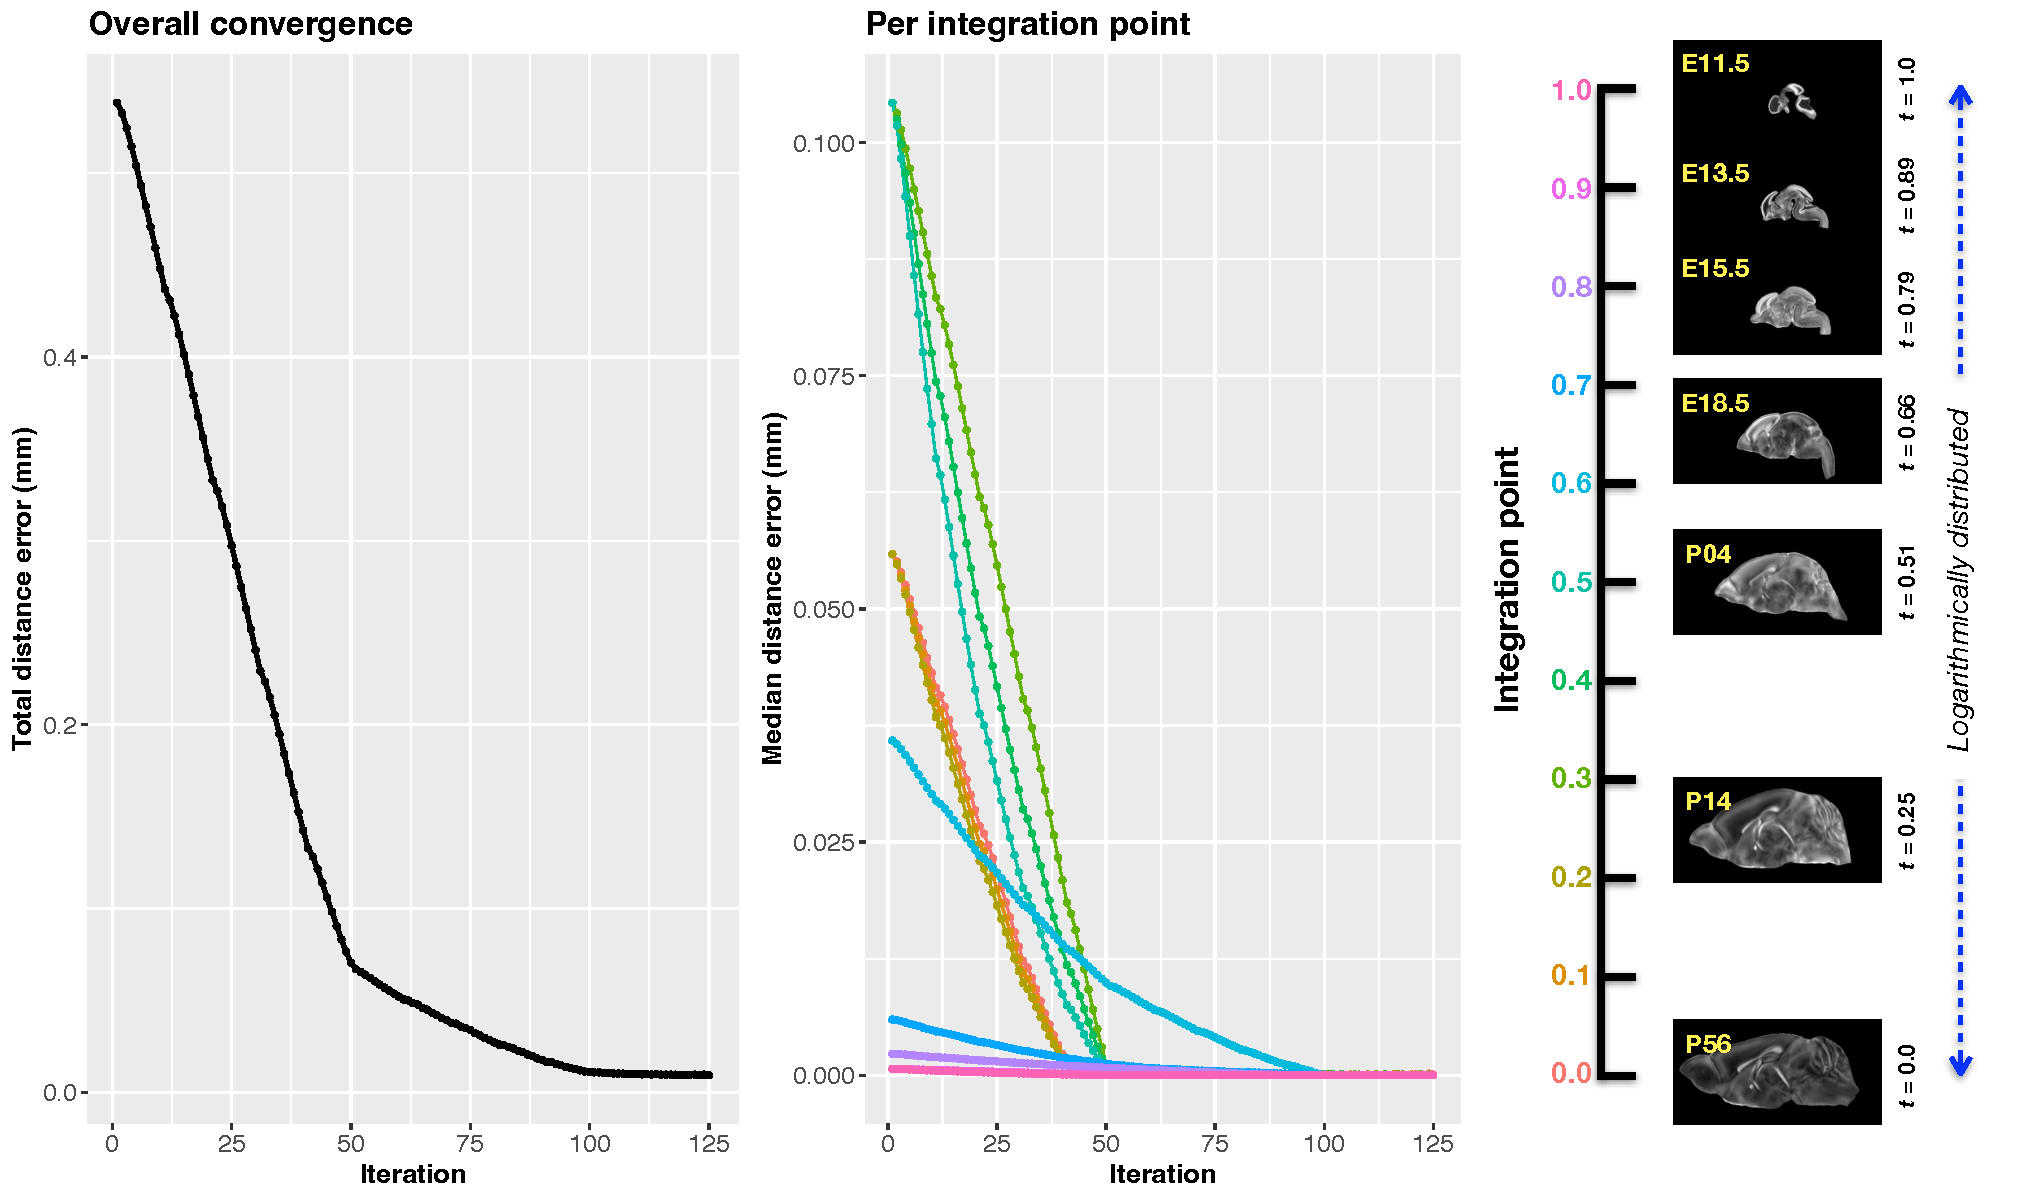
\includegraphics[width=0.99\textwidth]{Figures/convergence.pdf}
\caption{Convergence of the optimization of the velocity field for describing the 
transformation through the developmental stages from E11.5 through P56.}
\label{fig:convergence}
\end{figure}

\texttt{fit\_time\_varying\_transform\_to\_point\_sets(...)} from the
ANTsPy package was used to optimize the velocity field. Input comprised
the seven corresponding point sets and their associated weight values,
the selected number of integration points for the velocity field
(\(N=11\)), and the parameters defining the geometry of the spatial
dimensions of the velocity field (same as the downsampled P56 atlas
noted above). In addition, the normalized time point for each
atlas/point-set was also defined. Given the increasingly larger gaps in
the postnatal timepoint sampling, we made two adjustments. Based on
known mouse brain development, we used 28 days for the P56 data. We then
computed the log transform of the adjusted set of time points prior to
normalization between 0 and 1 (see the right side of Figure
\ref{fig:convergence}.) This log transform, as part of the temporal
normalization, significantly improved data spacing.

The max number of iterations was set to 200. At each iteration we looped
over the 11 integration points. At each integration point, the velocity
field estimate was updated by warping the two immediately adjacent point
sets to the integration time point and determining the regularized
displacement field between the two warped point sets. As with any
gradient-based descent algorithm, this field was multiplied by a small
step size (\(\delta = 0.2\)) before adding to the current velocity
field. Using multithreading, each iteration took about six minutes.

\begin{figure}[!htb]
\centering
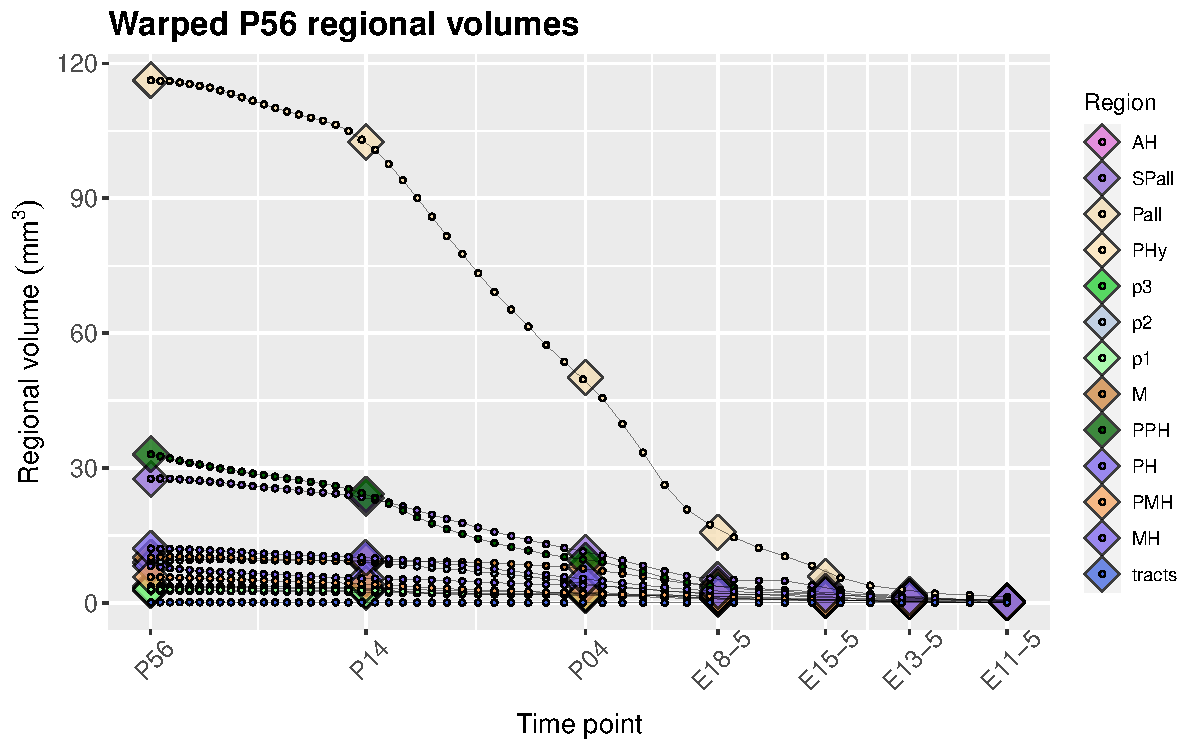
\includegraphics[width=0.75\textwidth]{Figures/warpedP56Volumes.pdf}
\caption{After the velocity field is generated, we can use it to warp
the simplified labels of the P56 atlas continuously over the interval
$[0, 1]$ and plot the volumes of the atlas regions.  Note how they 
compare with the volumes of the same regions in the other atlases.}
\label{fig:warpedP56}
\end{figure}

Convergence is determined by the average displacement error over each of
the integration points. As can be seen in the left panel of Figure
\ref{fig:convergence}, convergence occurred around 125 iterations when
the average displacement error is minimized. The median displacement
error at each of the integration points also trends towards zero but at
different rates. After optimization, we use the velocity field to warp
the P56 set of labels to each of the other atlas time points to compare
the volumes of the different simplified annotated regions. This is shown
in Figure \ref{fig:warpedP56}.

\hypertarget{the-devccf-transform-model}{%
\subsubsection*{The DevCCF transform
model}\label{the-devccf-transform-model}}
\addcontentsline{toc}{subsubsection}{The DevCCF transform model}

\begin{figure}[!htb]
\centering
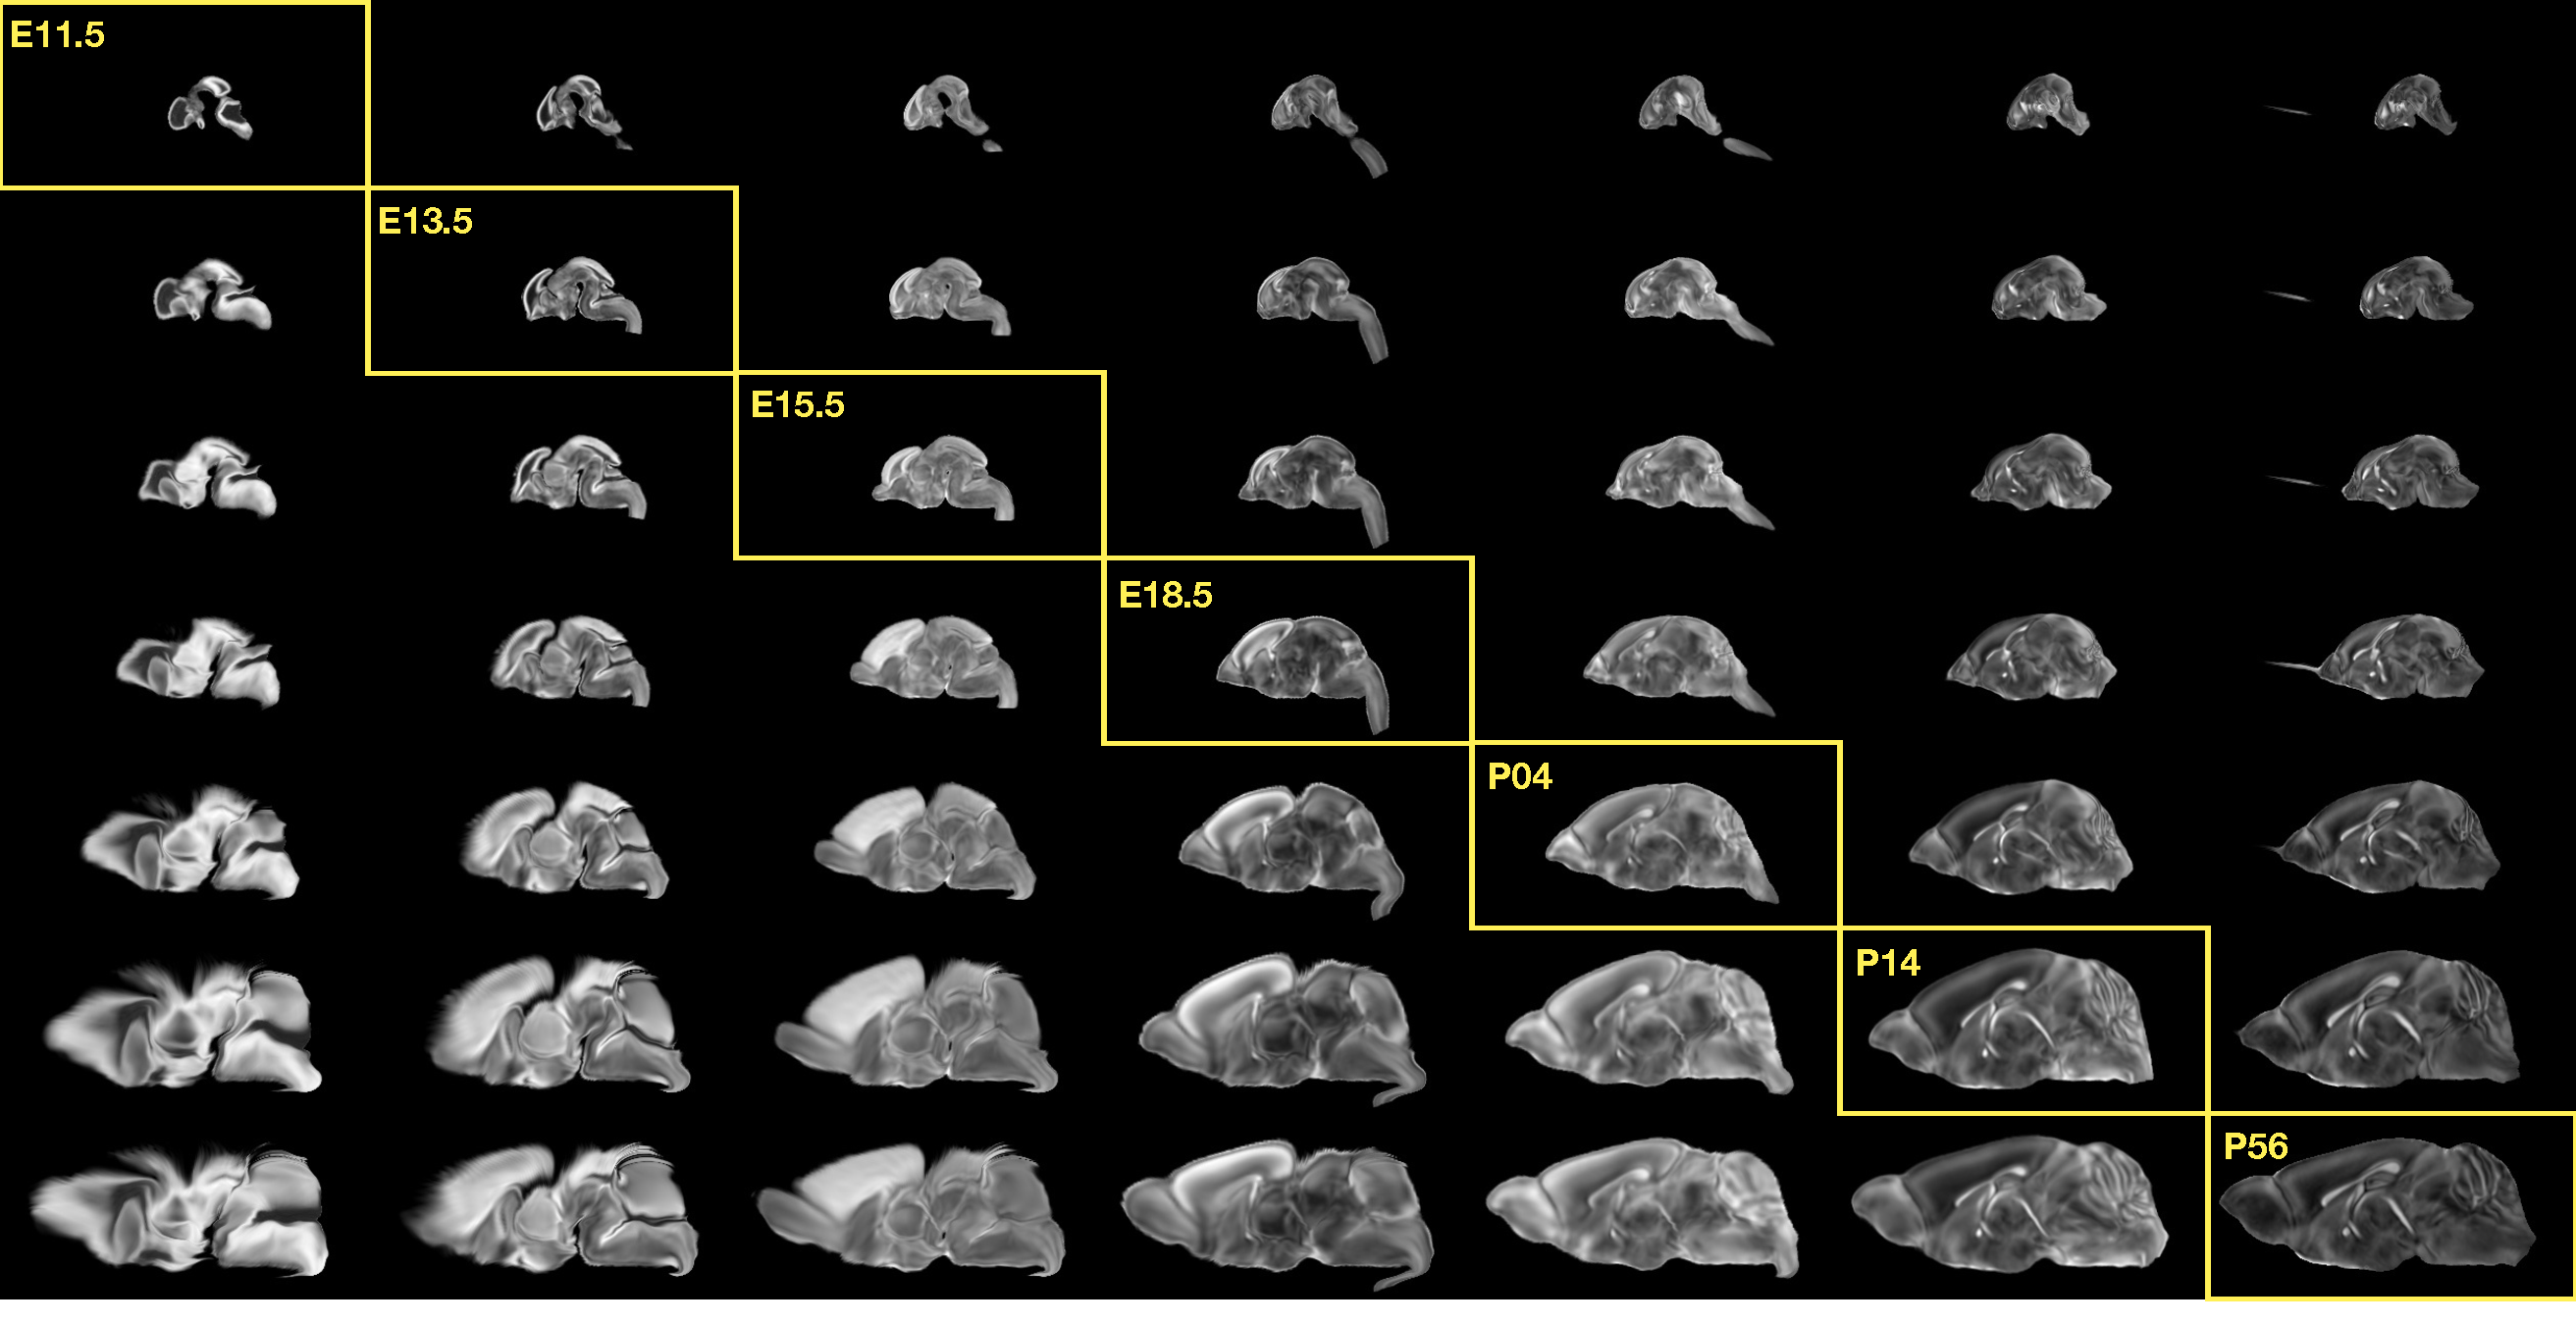
\includegraphics[width=0.99\textwidth]{Figures/CrossWarp.pdf}
\caption{Mid-sagittal visualization of the effects of the transformation model in
warping every developmental stage to the time point of every other developmental
stage.  The original images are located along the diagonal.  Columns correspond
to the warped original image whereas the rows represent the reference space to which
each image is warped.}
\label{fig:crosswarp}
\end{figure}

Once optimized, the resulting velocity field can be used to generate the
deformable transform between any two continuous points within the time
interval bounded by E11.5 and P56. So, for example, one can transform
each atlas to the space of every other atlas. This is illustrated in
Figure \ref{fig:crosswarp} where we render a mid-sagittal location for
each atlas and the results of warping every atlas to that space.

\begin{figure}[!htb]
\centering
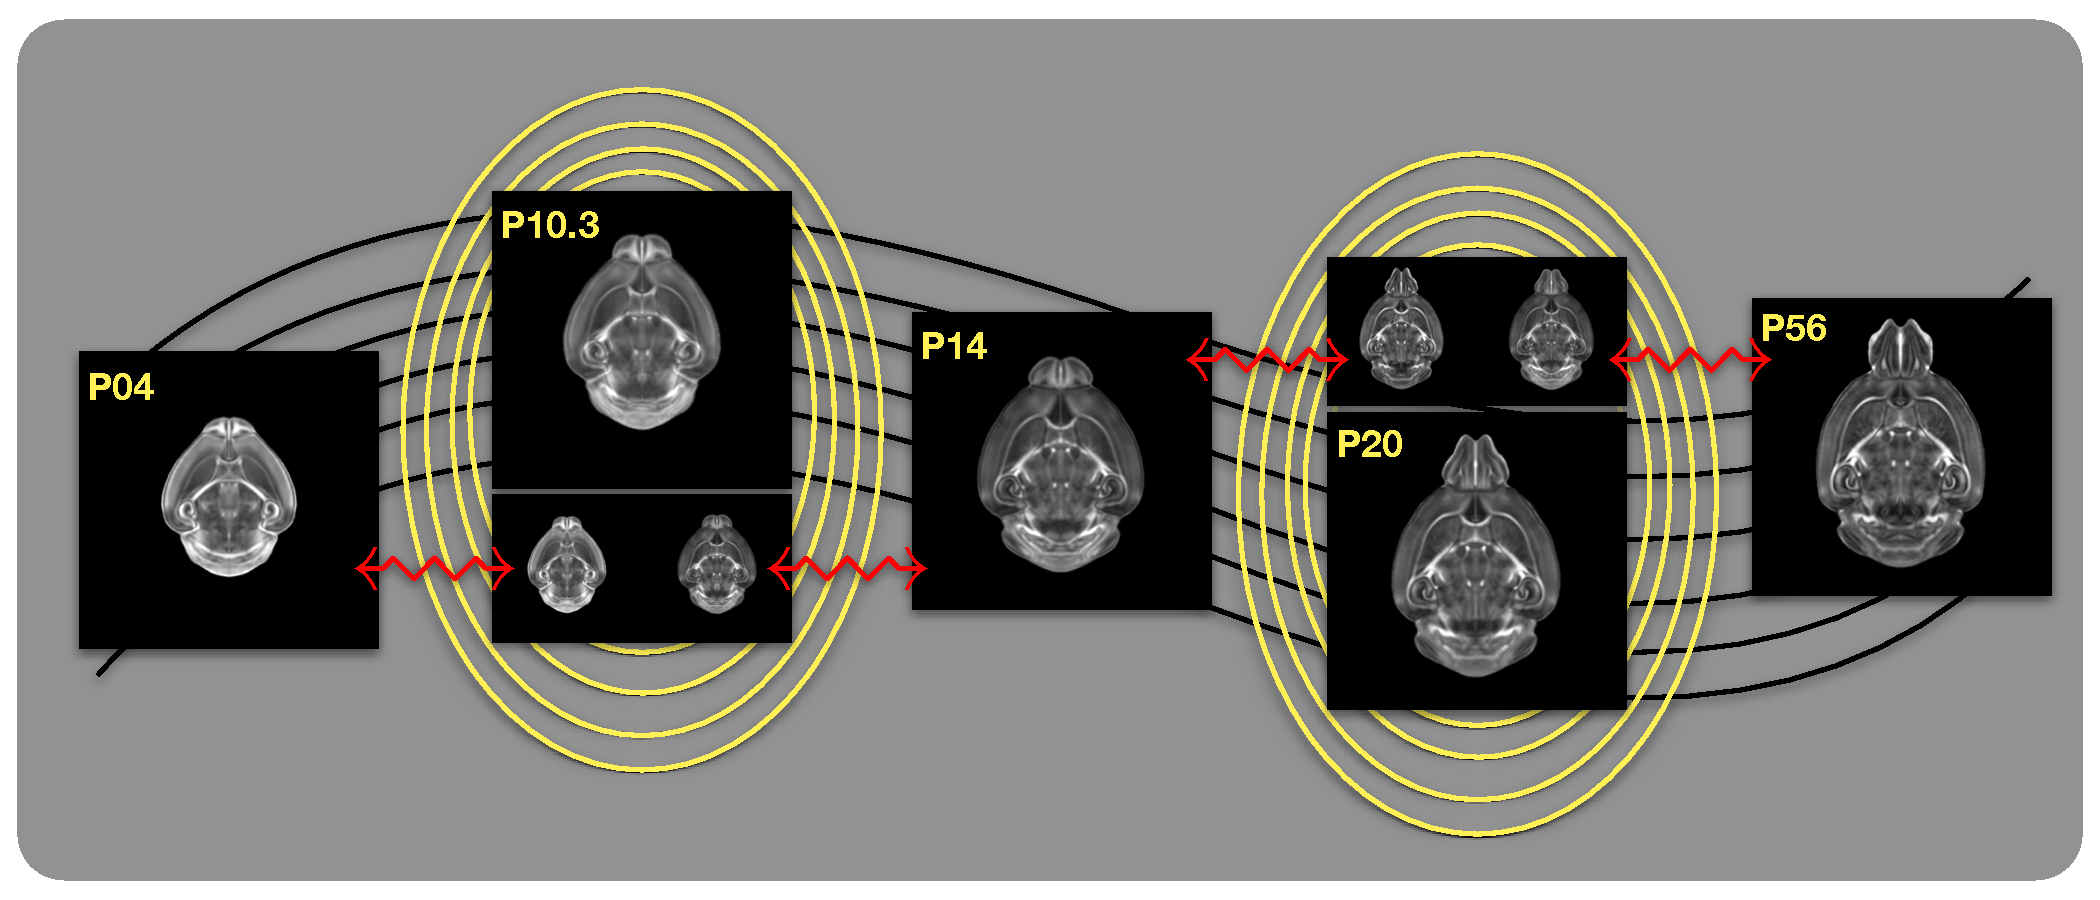
\includegraphics[width=0.99\textwidth]{Figures/pseudo_template.pdf}
\caption{Illustration of the use of the velocity flow model for creating pseudo-templates
at continuous time points not represented in one of the existing developmental stages.
For example, FA templates at time point P10.3 and P20 can be generated by warping the 
existing temporally adjacent developmental templates to the target time point and using 
those images in the ANTsX template building process.}
\label{fig:pseudo}
\end{figure}

One potential application for this particular transformation model is
facilitating the construction of pseudo-templates in the temporal gaps
of the DevCCF. This is illustrated in Figure \ref{fig:pseudo} where we
used the optimized velocity field to construct pseudo-templates at time
point P10.3 and P20---arbitrarily chosen simply to demonstrate the
concept. After situating these time points within the normalized time
point interval, the existing adjacent DevCCF atlases on either side can
be warped to the desired time point. A subsequent call to one of the
ANTsX template building functions then permits the construction of the
template at that time point. Note that both of these usage examples can
be found on the GitHub repository given above.

\clearpage
\newpage

\hypertarget{discussion}{%
\section*{Discussion}\label{discussion}}
\addcontentsline{toc}{section}{Discussion}

In this study, we employed precision mapping techniques and
high-resolution image acquisition to investigate the spatial
organization of gene activity and their interactions in the mouse brain.
Leveraging the Advanced Normalization Tools Ecosystem (ANTsX), an
open-source software image analysis toolkit, we demonstrated its utility
in generating precise spatial mappings of the mouse brain at different
developmental ages. The focus of this discussion is on the construction
and application of the DevCCF Velocity Flow Model, showcasing its
versatility and potential implications.

The velocity flow model was constructed to continuously link the
developmental atlases, providing a dynamic representation of the mouse
brain's transformation across different developmental stages. ANTsX,
built on the Insight Segmentation and Registration Toolkit (ITK),
facilitated the creation of a 4-D velocity field, employing a B-spline
scattered data approximation technique for field regularization. The
optimization of the velocity field was achieved through a unique
approach, involving iterative correspondence determination and
transformation optimization.

The choice of a velocity field size of \([256, 182, 360]\) with 11
integration points struck a balance between tractability, portability,
and accuracy. The resulting velocity field, though compact, encapsulated
the intricate changes across developmental stages, ensuring the
representativeness of the model. The entire process, including data
preparation and optimization, is well-documented and accessible through
a dedicated GitHub repository.

Data preparation involved the transformation of labeled annotations to a
common space, enabling the establishment of a common point set across
all developmental atlases. The optimization process included the rigid
transformation of data, determination of common point sets, and the
subsequent generation of the velocity field. The convergence of the
optimization process, illustrated in Figure \ref{fig:convergence},
highlighted the efficiency of the employed methodology.

The velocity field was further validated through the warping of
simplified labels, providing visual insights into the consistency and
accuracy of the model. The availability of the warped P56 atlas volumes,
as depicted in Figure \ref{fig:warpedP56}, enables a comprehensive
comparison of annotated regions across developmental stages.

The DevCCF transform model, once optimized, offers a powerful tool for
generating deformable transformations between any two continuous points
within the developmental time interval. This capability is exemplified
in Figure \ref{fig:crosswarp}, where each atlas is transformed to the
space of every other atlas, providing a detailed view of the
developmental trajectory.

An intriguing application of this transformation model is the creation
of pseudo-templates in temporal gaps within the DevCCF. As depicted in
Figure \ref{fig:pseudo}, the velocity flow model enables the generation
of templates at continuous time points not represented in existing
developmental stages. This novel application can significantly enhance
our understanding of intermediate developmental states.

In conclusion, the presented DevCCF Velocity Flow Model, constructed and
optimized using ANTsX, represents a valuable contribution to the field
of mouse brain mapping. The ability to continuously link developmental
atlases, visualize transformations, and generate pseudo-templates opens
avenues for in-depth explorations of gene activity and
structural-functional relationships during brain development. The
accessibility of the methodology and results through the provided GitHub
repository encourages further exploration and collaboration within the
scientific community. \clearpage \newpage

\hypertarget{methods}{%
\section*{Methods}\label{methods}}
\addcontentsline{toc}{section}{Methods}

\hypertarget{preprocessing-bias-field-correction-and-denoising}{%
\subsection*{Preprocessing: bias field correction and
denoising}\label{preprocessing-bias-field-correction-and-denoising}}
\addcontentsline{toc}{subsection}{Preprocessing: bias field correction
and denoising}

As in human studies, bias field correction and image denoising are
standard preprocessing steps in improving overall image quality in mouse
brain images. The bias field, a gradual spatial intensity variation in
images, can arise from various sources such as magnetic field
inhomogeneity or acquisition artifacts, leading to distortions that can
compromise the quality of brain images. Correcting for bias fields
ensures a more uniform and consistent representation of brain
structures, enabling accurate quantitative analysis. Additionally, brain
images are often susceptible to various forms of noise, which can
obscure subtle features and affect the precision of measurements.
Denoising techniques help mitigate the impact of noise, enhancing the
signal-to-noise ratio and improving the overall image quality. The
well-known N4 bias field correction algorithm\textsuperscript{24} has
its origins in the ANTs toolkit which was implemented and introduced
into the ITK toolkit. Similarly, ANTsX contains an implementation of a
well-performing patch-based denoising technique\textsuperscript{53} and
is also available as a image filter to the ITK community.

\hypertarget{antsxnet-mouse-brain-applications}{%
\subsection*{ANTsXNet mouse brain
applications}\label{antsxnet-mouse-brain-applications}}
\addcontentsline{toc}{subsection}{ANTsXNet mouse brain applications}

\emph{General notes regarding deep learning training.}

All network-based approaches described below were implemented and
organized in the ANTsXNet libraries comprising Python (ANTsPyNet) and R
(ANTsRNet) analogs using the Keras/Tensorflow libraries available as
open-source in ANTsX GitHub repositories. For the various applications,
both share the identically trained weights for mutual reproducibility.
Training data was provided by manual labeling by various co-authors and
expanded using both intensity-based and shape-based data augmentation
techniques.

Intensity-based data augmentation consisted of randomly added noise
based on ITK functionality, simulated bias fields based on N4 bias field
modeling, and histogram warping for mimicking well-known MRI intensity
nonlinearities.\textsuperscript{25,54} These augmentation techniques are
available in ANTsXNet (only ANTsPyNet versions are listed): simulated
bias field: \texttt{simulate\_bias\_field(...)}, image noise:
\texttt{add\_noise\_to\_image(...)}, and MRI intensity nonlinear
characterization: \texttt{histogram\_warp\_image\_intensities(...)}.
Shape-based data augmentation used both random linear and nonlinear
deformations. This functionality is also instantiated within ANTsXNet in
terms of random spatial warping:
\texttt{randomly\_transform\_image\_data(...)}.

For all GPU training, we used Python scripts for creating custom batch
generators. As such batch generators tend to be application-specific, we
store them in a separate GitHub repository for public availability
(\url{https://github.com/ntustison/ANTsXNetTraining}). In terms of GPU
hardware, all training was done on a DGX (GPUs: 4X Tesla V100, system
memory: 256 GB LRDIMM DDR4).

\emph{Brain extraction.}

Similar to human neuroimage processing, brain extraction is a crucial
preprocessing step for accurate brain mapping. Within ANTsXNet, we have
created several deep learning networks for brain extraction for several
image modalities (e.g., T1, FLAIR, fractional anisotropy). Similarly,
for the developmental brain atlas work\textsuperscript{47} we developed
similar functionality for mouse brains of different modalities and
developmental age. All networks use a conventional 2-D U-net
architecture\textsuperscript{55} and perform prediction in a slice-wise
fashion given the limitations of the acquisition protocols (e.g.,
missing slices, slice thickness). Currently, coronal and sagittal
networks are available for both E13.5 and E15.5 data and coronal network
for T2-weighted MRI. In ANTsPyNet, this functionality is available in
the program \texttt{brain\_extraction(...)}. Even when physical brain
extraction is performed prior to image acquisition, artifacts, such as
bubbles or debris, can complicate subsequent processing. Similar to the
brain extraction networks, a 2-D U-net architecture\textsuperscript{55}
was created to separate the background and foreground.

\emph{Miscellaneous networks: Super-resolution, cerebellum, and
hemispherical masking.}

To further enhance the data prior to designing mapping protocols,
additional networks were created. A well-performing deep back projection
network\textsuperscript{56} was ported to ANTsXNet and expanded to 3-D
for various super-resolution applications,\textsuperscript{57} including
mouse data. Finally, features of anatomical significance, namely the
cerebellum and hemispherical midline were captured in these data using
deep learning networks.

\hypertarget{intra-slice-image-registration-with-missing-slice-imputation}{%
\subsection*{Intra-slice image registration with missing slice
imputation}\label{intra-slice-image-registration-with-missing-slice-imputation}}
\addcontentsline{toc}{subsection}{Intra-slice image registration with
missing slice imputation}

Volumetric gene expression slice data was collated into 3-D volumes
using \ldots{} (ask Jeff). Prior to mapping this volume to the
corresponding structural data and, potentially, to the appropriate
template, alignment was improved using deformable registration on
contiguous slices. However, one of the complications associated with
these image data was the unknown number of missing slices, the number of
consecutive missing slices, and the different locations of these missing
slices. To handle this missing data problem, we found that data
interpolation using the B-spline approximation algorithm cited
earlier\textsuperscript{52} (ANTsPy function:
\texttt{fit\_bspline\_object\_to\_scattered\_data(...)}). This provided
sufficient data interpolation fidelity to perform continuous slicewise
registration. Other possible variants that were considered but deemed
unnecessary was performing more than one iteration cycling through data
interpolation and slicewise alignment. The other possibility was
incorporating the super-resolution technique described earlier. But
again, our data did not require these additional steps.

\hypertarget{image-registration}{%
\subsection*{Image registration}\label{image-registration}}
\addcontentsline{toc}{subsection}{Image registration}

The ANTs registration toolkit is a complex framework permitting highly
tailored solutions to pairwise image registration
scenarios.\textsuperscript{58} It includes innovative transformation
models for biological modeling\textsuperscript{39,59} and has proven
capable of excellent performance.\textsuperscript{40,60} Various
parameter sets targeting specific applications have been packaged with
the different ANTsX platforms, specifically ANTs, ANTsPy, and
ANTsR.\textsuperscript{25} In ANTsPy, the function
\texttt{ants.registration(...)} is used to register two (sets) of images
where \texttt{type\_of\_transform} is a user-specified option that
invokes a specific parameter set. Initially, linear optimization is
initialized with center of (intensity) mass alignment typically followed
by optimization of both rigid and affine transforms using the mutual
information similarity metric. This was followed by diffeomorphic
deformable alignment using symmetric normalization (SyN) with
Gaussian\textsuperscript{39} or B-spline
regularization\textsuperscript{59} where the forward transform is
invertible and differentiable. The similarity metric employed at this
latter stage is typically either neighborhood cross-correlation or
mutual information similarity metric. Further details can be found in
the various documentation sources for these ANTsX packages.

\hypertarget{template-generation}{%
\subsection*{Template generation}\label{template-generation}}
\addcontentsline{toc}{subsection}{Template generation}

ANTsX provides functionality for constructing templates from a set (or
multi-modal sets) of input images as originally
described\textsuperscript{50} and recently used to create the DevCCF
templates.\textsuperscript{47} An initial template estimate is
constructed from an existing subject image or a voxelwise average
derived from a rigid pre-alignment of the image population. Pairwise
registration between each subject and the current template estimate is
performed using the Symmetric Normalization (SyN)
algorithm.\textsuperscript{39} The template estimate is updated by
warping all subjects to the space of the template, performing a
voxelwise average, and then performing a ``shape update'' of this latter
image by warping it by the average inverse deformation, thus yielding a
mean image of the population in terms of both the intensity and shape.

\hypertarget{continuous-developmental-velocity-flow-transformation-model}{%
\subsection*{Continuous developmental velocity flow transformation
model}\label{continuous-developmental-velocity-flow-transformation-model}}
\addcontentsline{toc}{subsection}{Continuous developmental velocity flow
transformation model}

Given multiple, linearly or non-linearly ordered point sets where
individual points across are in one-to-one correspondence, we developed
an approach for generating a velocity flow transformation model to
describe a time-varying diffeomorphic mapping as a variant of the
inexact landmark matching solution of Joshi and
Miller.\textsuperscript{48} Integration of the resulting velocity field
can then be used to describe the displacement between any two time
points within this time-parameterized domain. Regularization of the
sparse correspondence between point sets is performed using a
generalized B-spline scattered data approximation
technique,\textsuperscript{52} also developed by the ANTsX developers
and contributed to ITK.

To apply this methodology to the developmental
templates,\textsuperscript{47} we coalesced the manual parcellations of
the developmental templates into 26 common anatomical regions (13 per
hemisphere). We then used these regions to generate invertible
transformations between successive time points. Specifically each label
was used to create a pair of single region images resulting in 26 pairs
of ``source'' and ``target'' images. The multiple image pairs were used
to iteratively estimate a diffeomorphic pairwise transform. Given the
seven atlases E11.5, E13.5, E15.5, E18.5, P4, P14, and P56, this
resulted in 6 sets of transforms between successive time points. Given
the relative sizes between atlases, on the order of 10\(^6\) points were
randomly sampled labelwise in the P56 template space and propagated to
each successive atlas providing the point sets for constructing the
velocity flow model. Approximately 200 iterations resulted in a steady
convergence based on the average Euclidean norm between transformed
point sets. Ten integration points were used and point sets were
distributed along the temporal dimension using a log transform for a
more evenly spaced sampling. Further details including links to data and
scripts to reproduce our reported results is found in the associated
GitHub repository.

\hypertarget{visualization}{%
\subsection*{Visualization}\label{visualization}}
\addcontentsline{toc}{subsection}{Visualization}

To complement the well-known visualization capabilities of R and Python,
e.g., ggplot2 and matplotlib, respectively, image-specific visualization
capabilities are available in the \texttt{ants.plot(...)} (Python) and
\texttt{plot.antsImage(...)} (R). These are capable of illustrating
multiple slices in different orientations with both other image overlays
as well as label images.

\clearpage
\newpage

\textbf{Data availability.} All data used in this work are publicly
available. The DevCCF atlas is available at
\url{https://kimlab.io/brain-map/DevCCF/}. Additionally, all software
discussed is publicly available. ANTsPy and ANTsR are available through
GitHub at the ANTsX Ecosystem (\url{https://github.com/ANTsX}). A GitHub
repository specific to the work discussed in the manuscript was created
and is available at
\url{https://github.com/ntustison/DevCCF-Velocity-Flow}.

\clearpage

\hypertarget{references}{%
\section*{References}\label{references}}
\addcontentsline{toc}{section}{References}

\hypertarget{refs}{}
\begin{CSLReferences}{0}{0}
\leavevmode\vadjust pre{\hypertarget{ref-Keller:2015aa}{}}%
\CSLLeftMargin{1. }
\CSLRightInline{Keller, P. J. \& Ahrens, M. B. Visualizing whole-brain
activity and development at the single-cell level using light-sheet
microscopy. \emph{Neuron} \textbf{85}, 462--83 (2015).}

\leavevmode\vadjust pre{\hypertarget{ref-La-Manno:2021aa}{}}%
\CSLLeftMargin{2. }
\CSLRightInline{La Manno, G. \emph{et al.} Molecular architecture of the
developing mouse brain. \emph{Nature} \textbf{596}, 92--96 (2021).}

\leavevmode\vadjust pre{\hypertarget{ref-Wen:2022aa}{}}%
\CSLLeftMargin{3. }
\CSLRightInline{Wen, L. \emph{et al.} Single-cell technologies: From
research to application. \emph{Innovation (Camb)} \textbf{3}, 100342
(2022).}

\leavevmode\vadjust pre{\hypertarget{ref-Oh:2014aa}{}}%
\CSLLeftMargin{4. }
\CSLRightInline{Oh, S. W. \emph{et al.} A mesoscale connectome of the
mouse brain. \emph{Nature} \textbf{508}, 207--14 (2014).}

\leavevmode\vadjust pre{\hypertarget{ref-Gong:2013aa}{}}%
\CSLLeftMargin{5. }
\CSLRightInline{Gong, H. \emph{et al.} Continuously tracing brain-wide
long-distance axonal projections in mice at a one-micron voxel
resolution. \emph{Neuroimage} \textbf{74}, 87--98 (2013).}

\leavevmode\vadjust pre{\hypertarget{ref-Li:2010aa}{}}%
\CSLLeftMargin{6. }
\CSLRightInline{Li, A. \emph{et al.} Micro-optical sectioning tomography
to obtain a high-resolution atlas of the mouse brain. \emph{Science}
\textbf{330}, 1404--8 (2010).}

\leavevmode\vadjust pre{\hypertarget{ref-Ueda:2020aa}{}}%
\CSLLeftMargin{7. }
\CSLRightInline{Ueda, H. R. \emph{et al.} Tissue clearing and its
applications in neuroscience. \emph{Nat Rev Neurosci} \textbf{21},
61--79 (2020).}

\leavevmode\vadjust pre{\hypertarget{ref-Stahl:2016aa}{}}%
\CSLLeftMargin{8. }
\CSLRightInline{Ståhl, P. L. \emph{et al.} Visualization and analysis of
gene expression in tissue sections by spatial transcriptomics.
\emph{Science} \textbf{353}, 78--82 (2016).}

\leavevmode\vadjust pre{\hypertarget{ref-Burgess:2019aa}{}}%
\CSLLeftMargin{9. }
\CSLRightInline{Burgess, D. J. Spatial transcriptomics coming of age.
\emph{Nat Rev Genet} \textbf{20}, 317 (2019).}

\leavevmode\vadjust pre{\hypertarget{ref-MacKenzie-Graham:2004aa}{}}%
\CSLLeftMargin{10. }
\CSLRightInline{MacKenzie-Graham, A. \emph{et al.} A multimodal,
multidimensional atlas of the C57BL/6J mouse brain. \emph{J Anat}
\textbf{204}, 93--102 (2004).}

\leavevmode\vadjust pre{\hypertarget{ref-Mackenzie-Graham:2007aa}{}}%
\CSLLeftMargin{11. }
\CSLRightInline{Mackenzie-Graham, A. J. \emph{et al.} Multimodal,
multidimensional models of mouse brain. \emph{Epilepsia} \textbf{48
Suppl 4}, 75--81 (2007).}

\leavevmode\vadjust pre{\hypertarget{ref-Dong:2008aa}{}}%
\CSLLeftMargin{12. }
\CSLRightInline{Dong, H. W. \emph{Allen reference atlas. A digital color
brain atlas of the C57BL/6J male mouse}. (John Wiley; Sons, 2008).}

\leavevmode\vadjust pre{\hypertarget{ref-Wang:2020aa}{}}%
\CSLLeftMargin{13. }
\CSLRightInline{Wang, Q. \emph{et al.} The allen mouse brain common
coordinate framework: A 3D reference atlas. \emph{Cell} \textbf{181},
936--953.e20 (2020).}

\leavevmode\vadjust pre{\hypertarget{ref-Johnson:2010aa}{}}%
\CSLLeftMargin{14. }
\CSLRightInline{Johnson, G. A. \emph{et al.} Waxholm space: An
image-based reference for coordinating mouse brain research.
\emph{Neuroimage} \textbf{53}, 365--72 (2010).}

\leavevmode\vadjust pre{\hypertarget{ref-Oguz:2014aa}{}}%
\CSLLeftMargin{15. }
\CSLRightInline{Oguz, I., Zhang, H., Rumple, A. \& Sonka, M. RATS: Rapid
automatic tissue segmentation in rodent brain MRI. \emph{J Neurosci
Methods} \textbf{221}, 175--82 (2014).}

\leavevmode\vadjust pre{\hypertarget{ref-Sawiak:2014aa}{}}%
\CSLLeftMargin{16. }
\CSLRightInline{Sawiak, S. J., Picq, J.-L. \& Dhenain, M. Voxel-based
morphometry analyses of in vivo MRI in the aging mouse lemur primate.
\emph{Front Aging Neurosci} \textbf{6}, 82 (2014).}

\leavevmode\vadjust pre{\hypertarget{ref-Ashburner:2012aa}{}}%
\CSLLeftMargin{17. }
\CSLRightInline{Ashburner, J. {SPM}: A history. \emph{Neuroimage}
\textbf{62}, 791--800 (2012).}

\leavevmode\vadjust pre{\hypertarget{ref-Modat:2010aa}{}}%
\CSLLeftMargin{18. }
\CSLRightInline{Modat, M. \emph{et al.} Fast free-form deformation using
graphics processing units. \emph{Comput Methods Programs Biomed}
\textbf{98}, 278--84 (2010).}

\leavevmode\vadjust pre{\hypertarget{ref-Tyson:2022aa}{}}%
\CSLLeftMargin{19. }
\CSLRightInline{Tyson, A. L. \emph{et al.} Accurate determination of
marker location within whole-brain microscopy images. \emph{Sci Rep}
\textbf{12}, 867 (2022).}

\leavevmode\vadjust pre{\hypertarget{ref-Pallast:2019aa}{}}%
\CSLLeftMargin{20. }
\CSLRightInline{Pallast, N. \emph{et al.} Processing pipeline for
atlas-based imaging data analysis of structural and functional mouse
brain MRI (AIDAmri). \emph{Front Neuroinform} \textbf{13}, 42 (2019).}

\leavevmode\vadjust pre{\hypertarget{ref-Jenkinson:2012wi}{}}%
\CSLLeftMargin{21. }
\CSLRightInline{Jenkinson, M., Beckmann, C. F., Behrens, T. E. J.,
Woolrich, M. W. \& Smith, S. M. FSL. \emph{Neuroimage} \textbf{62},
782--90 (2012).}

\leavevmode\vadjust pre{\hypertarget{ref-Yeh:2010aa}{}}%
\CSLLeftMargin{22. }
\CSLRightInline{Yeh, F.-C., Wedeen, V. J. \& Tseng, W.-Y. I. Generalized
q-sampling imaging. \emph{IEEE Trans Med Imaging} \textbf{29}, 1626--35
(2010).}

\leavevmode\vadjust pre{\hypertarget{ref-Jorge-Cardoso:2013aa}{}}%
\CSLLeftMargin{23. }
\CSLRightInline{Jorge Cardoso, M. \emph{et al.} STEPS: Similarity and
truth estimation for propagated segmentations and its application to
hippocampal segmentation and brain parcelation. \emph{Med Image Anal}
\textbf{17}, 671--84 (2013).}

\leavevmode\vadjust pre{\hypertarget{ref-Tustison:2010ac}{}}%
\CSLLeftMargin{24. }
\CSLRightInline{Tustison, N. J. \emph{et al.} {N4ITK}: Improved {N3}
bias correction. \emph{IEEE Trans Med Imaging} \textbf{29}, 1310--20
(2010).}

\leavevmode\vadjust pre{\hypertarget{ref-Tustison:2021aa}{}}%
\CSLLeftMargin{25. }
\CSLRightInline{Tustison, N. J. \emph{et al.} The ANTsX ecosystem for
quantitative biological and medical imaging. \emph{Sci Rep} \textbf{11},
9068 (2021).}

\leavevmode\vadjust pre{\hypertarget{ref-Goubran:2019aa}{}}%
\CSLLeftMargin{26. }
\CSLRightInline{Goubran, M. \emph{et al.} Multimodal image registration
and connectivity analysis for integration of connectomic data from
microscopy to MRI. \emph{Nat Commun} \textbf{10}, 5504 (2019).}

\leavevmode\vadjust pre{\hypertarget{ref-Celestine:2020aa}{}}%
\CSLLeftMargin{27. }
\CSLRightInline{Celestine, M., Nadkarni, N. A., Garin, C. M., Bougacha,
S. \& Dhenain, M. Sammba-MRI: A library for processing SmAll-MaMmal
BrAin MRI data in python. \emph{Front Neuroinform} \textbf{14}, 24
(2020).}

\leavevmode\vadjust pre{\hypertarget{ref-Ioanas:2021aa}{}}%
\CSLLeftMargin{28. }
\CSLRightInline{Ioanas, H.-I., Marks, M., Zerbi, V., Yanik, M. F. \&
Rudin, M. An optimized registration workflow and standard geometric
space for small animal brain imaging. \emph{Neuroimage} \textbf{241},
118386 (2021).}

\leavevmode\vadjust pre{\hypertarget{ref-Cox:2012aa}{}}%
\CSLLeftMargin{29. }
\CSLRightInline{Cox, R. W. {AFNI}: What a long strange trip it's been.
\emph{Neuroimage} \textbf{62}, 743--7 (2012).}

\leavevmode\vadjust pre{\hypertarget{ref-Ni:2020aa}{}}%
\CSLLeftMargin{30. }
\CSLRightInline{Ni, H. \emph{et al.} A robust image registration
interface for large volume brain atlas. \emph{Sci Rep} \textbf{10}, 2139
(2020).}

\leavevmode\vadjust pre{\hypertarget{ref-Jin:2022aa}{}}%
\CSLLeftMargin{31. }
\CSLRightInline{Jin, M. \emph{et al.} SMART: An open-source extension of
WholeBrain for intact mouse brain registration and segmentation.
\emph{eNeuro} \textbf{9}, (2022).}

\leavevmode\vadjust pre{\hypertarget{ref-Furth:2018aa}{}}%
\CSLLeftMargin{32. }
\CSLRightInline{Fürth, D. \emph{et al.} An interactive framework for
whole-brain maps at cellular resolution. \emph{Nat Neurosci}
\textbf{21}, 139--149 (2018).}

\leavevmode\vadjust pre{\hypertarget{ref-Negwer:2022aa}{}}%
\CSLLeftMargin{33. }
\CSLRightInline{Negwer, M. \emph{et al.} FriendlyClearMap: An optimized
toolkit for mouse brain mapping and analysis. \emph{Gigascience}
\textbf{12}, (2022).}

\leavevmode\vadjust pre{\hypertarget{ref-Klein:2010aa}{}}%
\CSLLeftMargin{34. }
\CSLRightInline{Klein, S., Staring, M., Murphy, K., Viergever, M. A. \&
Pluim, J. P. W. Elastix: A toolbox for intensity-based medical image
registration. \emph{IEEE Trans Med Imaging} \textbf{29}, 196--205
(2010).}

\leavevmode\vadjust pre{\hypertarget{ref-Carey:2023aa}{}}%
\CSLLeftMargin{35. }
\CSLRightInline{Carey, H. \emph{et al.} DeepSlice: Rapid fully automatic
registration of mouse brain imaging to a volumetric atlas. \emph{Nat
Commun} \textbf{14}, 5884 (2023).}

\leavevmode\vadjust pre{\hypertarget{ref-Bajcsy:1982aa}{}}%
\CSLLeftMargin{36. }
\CSLRightInline{Bajcsy, R. \& Broit, C. Matching of deformed images. in
\emph{{S}ixth {I}nternational {C}onference on {P}attern {R}ecognition
({ICPR}'82)} 351--353 (1982).}

\leavevmode\vadjust pre{\hypertarget{ref-Bajcsy:1989aa}{}}%
\CSLLeftMargin{37. }
\CSLRightInline{Bajcsy, R. \& Kovacic, S. Multiresolution elastic
matching. \emph{Computer Vision, Graphics, and Image Processing}
\textbf{46}, 1--21 (1989).}

\leavevmode\vadjust pre{\hypertarget{ref-Gee:2003aa}{}}%
\CSLLeftMargin{38. }
\CSLRightInline{Gee, J., Sundaram, T., Hasegawa, I., Uematsu, H. \&
Hatabu, H. Characterization of regional pulmonary mechanics from serial
magnetic resonance imaging data. \emph{Acad Radiol} \textbf{10},
1147--52 (2003).}

\leavevmode\vadjust pre{\hypertarget{ref-Avants:2008aa}{}}%
\CSLLeftMargin{39. }
\CSLRightInline{Avants, B. B., Epstein, C. L., Grossman, M. \& Gee, J.
C. Symmetric diffeomorphic image registration with cross-correlation:
Evaluating automated labeling of elderly and neurodegenerative brain.
\emph{Med Image Anal} \textbf{12}, 26--41 (2008).}

\leavevmode\vadjust pre{\hypertarget{ref-Klein:2009aa}{}}%
\CSLLeftMargin{40. }
\CSLRightInline{Klein, A. \emph{et al.} Evaluation of 14 nonlinear
deformation algorithms applied to human brain {MRI} registration.
\emph{Neuroimage} \textbf{46}, 786--802 (2009).}

\leavevmode\vadjust pre{\hypertarget{ref-Murphy:2011aa}{}}%
\CSLLeftMargin{41. }
\CSLRightInline{Murphy, K. \emph{et al.} Evaluation of registration
methods on thoracic {CT}: The {EMPIRE10} challenge. \emph{IEEE Trans Med
Imaging} \textbf{30}, 1901--20 (2011).}

\leavevmode\vadjust pre{\hypertarget{ref-Baheti:2021aa}{}}%
\CSLLeftMargin{42. }
\CSLRightInline{Baheti, B. \emph{et al.} The brain tumor sequence
registration challenge: Establishing correspondence between
pre-operative and follow-up MRI scans of diffuse glioma patients.
(2021).}

\leavevmode\vadjust pre{\hypertarget{ref-Wang:2013ab}{}}%
\CSLLeftMargin{43. }
\CSLRightInline{Wang, H. \emph{et al.} Multi-atlas segmentation with
joint label fusion. \emph{IEEE Trans Pattern Anal Mach Intell}
\textbf{35}, 611--23 (2013).}

\leavevmode\vadjust pre{\hypertarget{ref-Tustison:2014aa}{}}%
\CSLLeftMargin{44. }
\CSLRightInline{Tustison, N. J. \emph{et al.} Optimal symmetric
multimodal templates and concatenated random forests for supervised
brain tumor segmentation (simplified) with {\(ANTsR\)}.
\emph{Neuroinformatics} (2014)
doi:\href{https://doi.org/10.1007/s12021-014-9245-2}{10.1007/s12021-014-9245-2}.}

\leavevmode\vadjust pre{\hypertarget{ref-Tustison:2015ab}{}}%
\CSLLeftMargin{45. }
\CSLRightInline{Tustison, N. J., Yang, Y. \& Salerno, M. Advanced
normalization tools for cardiac motion correction. in \emph{Statistical
atlases and computational models of the heart - imaging and modelling
challenges} (eds. Camara, O. et al.) vol. 8896 3--12 (Springer
International Publishing, 2015).}

\leavevmode\vadjust pre{\hypertarget{ref-McCormick:2014aa}{}}%
\CSLLeftMargin{46. }
\CSLRightInline{McCormick, M., Liu, X., Jomier, J., Marion, C. \&
Ibanez, L. ITK: Enabling reproducible research and open science.
\emph{Front Neuroinform} \textbf{8}, 13 (2014).}

\leavevmode\vadjust pre{\hypertarget{ref-Kronman:2023aa}{}}%
\CSLLeftMargin{47. }
\CSLRightInline{Kronman, F. A. \emph{et al.} Developmental mouse brain
common coordinate framework. \emph{bioRxiv} (2023)
doi:\href{https://doi.org/10.1101/2023.09.14.557789}{10.1101/2023.09.14.557789}.}

\leavevmode\vadjust pre{\hypertarget{ref-Joshi:2000aa}{}}%
\CSLLeftMargin{48. }
\CSLRightInline{Joshi, S. C. \& Miller, M. I. Landmark matching via
large deformation diffeomorphisms. \emph{IEEE Trans Image Process}
\textbf{9}, 1357--70 (2000).}

\leavevmode\vadjust pre{\hypertarget{ref-Christensen:1996aa}{}}%
\CSLLeftMargin{49. }
\CSLRightInline{Christensen, G. E., Rabbitt, R. D. \& Miller, M. I.
Deformable templates using large deformation kinematics. \emph{IEEE
Trans Image Process} \textbf{5}, 1435--47 (1996).}

\leavevmode\vadjust pre{\hypertarget{ref-Avants:2010aa}{}}%
\CSLLeftMargin{50. }
\CSLRightInline{Avants, B. B. \emph{et al.} The optimal template effect
in hippocampus studies of diseased populations. \emph{Neuroimage}
\textbf{49}, 2457--66 (2010).}

\leavevmode\vadjust pre{\hypertarget{ref-Tustison:2015vl}{}}%
\CSLLeftMargin{51. }
\CSLRightInline{Tustison, N. J. \emph{et al.} Optimal symmetric
multimodal templates and concatenated random forests for supervised
brain tumor segmentation (simplified) with ANTsR.
\emph{Neuroinformatics} \textbf{13}, 209--25 (2015).}

\leavevmode\vadjust pre{\hypertarget{ref-Tustison:2006aa}{}}%
\CSLLeftMargin{52. }
\CSLRightInline{Tustison, N. J. \& Amini, A. A. Biventricular myocardial
strains via nonrigid registration of anatomical {NURBS} model
{[}corrected{]}. \emph{IEEE Trans Med Imaging} \textbf{25}, 94--112
(2006).}

\leavevmode\vadjust pre{\hypertarget{ref-Manjon:2010aa}{}}%
\CSLLeftMargin{53. }
\CSLRightInline{Manjón, J. V., Coupé, P., Martí-Bonmatí, L., Collins, D.
L. \& Robles, M. Adaptive non-local means denoising of {MR} images with
spatially varying noise levels. \emph{J Magn Reson Imaging} \textbf{31},
192--203 (2010).}

\leavevmode\vadjust pre{\hypertarget{ref-Nyul:2000aa}{}}%
\CSLLeftMargin{54. }
\CSLRightInline{Nyúl, L. G., Udupa, J. K. \& Zhang, X. New variants of a
method of MRI scale standardization. \emph{IEEE Trans Med Imaging}
\textbf{19}, 143--50 (2000).}

\leavevmode\vadjust pre{\hypertarget{ref-Falk:2019aa}{}}%
\CSLLeftMargin{55. }
\CSLRightInline{Falk, T. \emph{et al.} U-net: Deep learning for cell
counting, detection, and morphometry. \emph{Nat Methods} \textbf{16},
67--70 (2019).}

\leavevmode\vadjust pre{\hypertarget{ref-Haris:2018aa}{}}%
\CSLLeftMargin{56. }
\CSLRightInline{Haris, M., Shakhnarovich, G. \& Ukita, N. Deep
back-projection networks for super-resolution. in \emph{2018 {IEEE/CVF}
{C}onference on {C}omputer {V}ision and {P}attern {R}ecognition}
1664--1673 (2018).
doi:\href{https://doi.org/10.1109/CVPR.2018.00179}{10.1109/CVPR.2018.00179}.}

\leavevmode\vadjust pre{\hypertarget{ref-Avants:2023aa}{}}%
\CSLLeftMargin{57. }
\CSLRightInline{Avants, B. B. \emph{et al.} Concurrent 3D super
resolution on intensity and segmentation maps improves detection of
structural effects in neurodegenerative disease. \emph{medRxiv} (2023)
doi:\href{https://doi.org/10.1101/2023.02.02.23285376}{10.1101/2023.02.02.23285376}.}

\leavevmode\vadjust pre{\hypertarget{ref-Avants:2014aa}{}}%
\CSLLeftMargin{58. }
\CSLRightInline{Avants, B. B. \emph{et al.} The {Insight} {ToolKit}
image registration framework. \emph{Front Neuroinform} \textbf{8}, 44
(2014).}

\leavevmode\vadjust pre{\hypertarget{ref-Tustison:2013ac}{}}%
\CSLLeftMargin{59. }
\CSLRightInline{Tustison, N. J. \& Avants, B. B. Explicit {B}-spline
regularization in diffeomorphic image registration. \emph{Front
Neuroinform} \textbf{7}, 39 (2013).}

\leavevmode\vadjust pre{\hypertarget{ref-Avants:2011wx}{}}%
\CSLLeftMargin{60. }
\CSLRightInline{Avants, B. B. \emph{et al.} A reproducible evaluation of
ANTs similarity metric performance in brain image registration.
\emph{Neuroimage} \textbf{54}, 2033--44 (2011).}

\end{CSLReferences}

\end{document}
